\documentclass[a2paper, 12pt]{article}
\usepackage[font={huge, bf}]{caption}
\usepackage{fontspec}
\setmainfont{Arial}
\usepackage{subcaption}
\usepackage{graphicx}
\usepackage{tikz}
\usepackage{tikzsymbols}
\usetikzlibrary{calc,patterns,shapes.geometric}
\usepackage{float}
\usepackage{pdflscape}
\usepackage{geometry}
\geometry{landscape, margin=2cm}
\captionsetup[subfigure]{justification=justified,singlelinecheck=false}
\pagestyle{empty}

\def\centerarc[#1](#2)(#3:#4:#5){\draw[#1] ($(#2)+({#5*cos(#3)},{#5*sin(#3)})$) arc (#3:#4:#5);}

\begin{document}
	\vspace*{\fill}
	\begin{figure}[!htbp]
		\centering
		\begin{subfigure}[b]{0.48\textwidth}
			\caption{Figure 1}
			\centering
			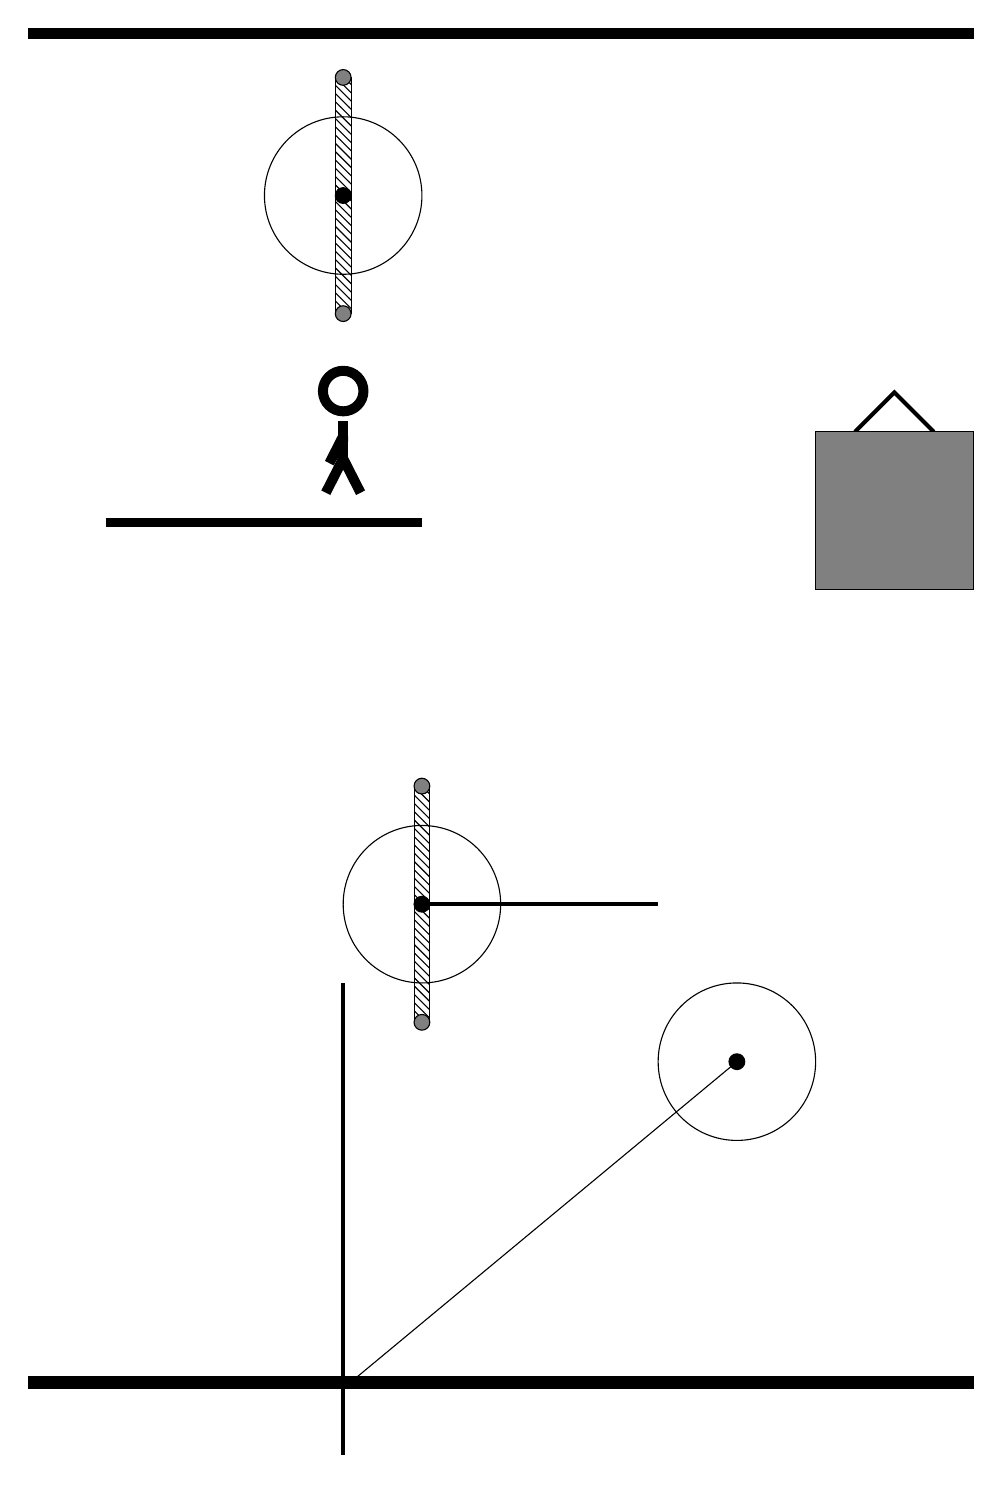
\begin{tikzpicture}
				\draw[fill=black] (-4, 14) rectangle (8, 14.125);
				
				\draw (5,1) circle (1);
				\draw[fill=black] (5,1) circle (0.1);
				\draw (0,-3.15) -- (5,1);
				
				\draw (0,12) circle (1);
				\draw[fill=black] (0,12) circle (0.1);
				\draw[pattern=north west lines, pattern color=black] (-0.1,13.5) rectangle (0.1,10.5);
				\draw[fill=black!50] (0,13.5) circle (0.1);
				\draw[fill=black!50] (0,10.5) circle (0.1);
				
				\draw (1,3) circle (1);
				\draw[fill=black] (1,3) circle (0.1);
				\draw[pattern=north west lines, pattern color=black] (0.9,4.5) rectangle (1.1,1.5);
				\draw[fill=black!50] (1,4.5) circle (0.1);
				\draw[fill=black!50] (1,1.5) circle (0.1);
				
				\draw[line width=0.5mm](6.5,9) --  (7,9.5) -- (7.5,9);
				\draw[fill=black!50] (6, 9) rectangle (8, 7);
				
				\draw[line width = 0.5mm] (1,3) -- (4,3);
				\centerarc[line width = 0.5mm](1,2)(90:180:1);
				\draw[line width = 0.5mm] (0,2) -- (0,-4);
				\centerarc[line width = 0.5mm](1,-4)(180:360:1);
				
				\node at (0, 9) {\scriptsize \Strichmaxerl[10][63][-92]};
				\draw[fill=black] (-3, 7.9) rectangle (1, 7.8);
				
				\draw[fill=black] (-4, -3) rectangle (8, -3.15);
			\end{tikzpicture}
		\end{subfigure}
		\hfill
		\begin{subfigure}[b]{0.48\textwidth}
			\caption{Figure 2}
			\centering
			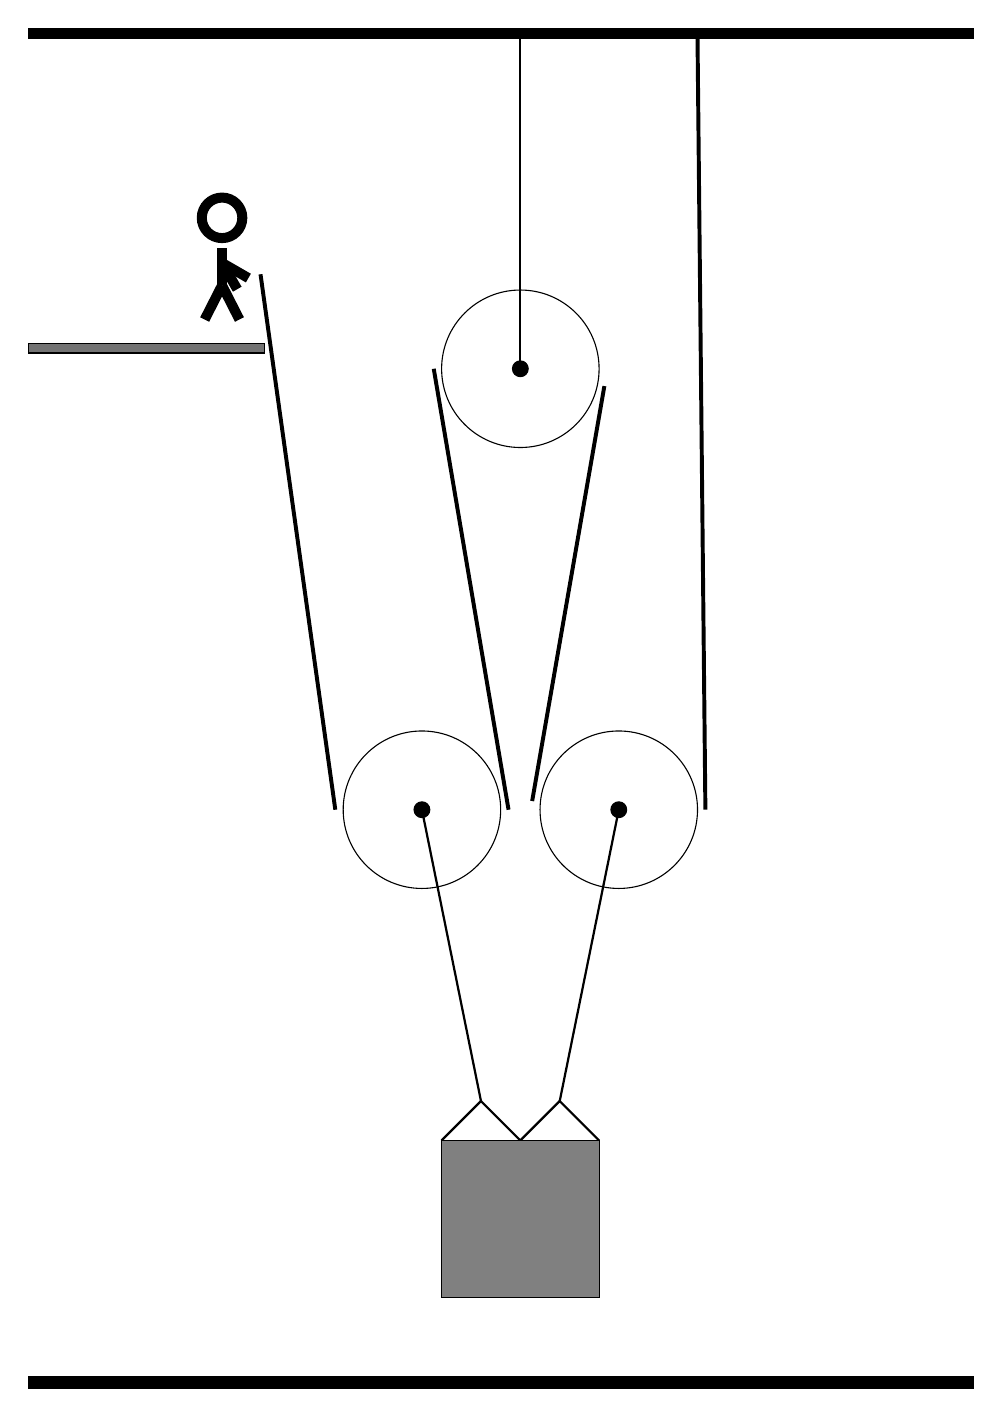
\begin{tikzpicture}
				\draw[fill=black] (-4, 14) rectangle (8, 14.125);
				
				\draw (1, 4.2) circle (1);
				\draw[fill=black] (1, 4.2) circle (0.1);
				
				\draw (2.25, 9.8) circle (1);
				\draw[fill=black] (2.25, 9.8) circle (0.1);
				\draw[thick] (2.25, 9.8) -- (2.25, 14);
				
				\draw (3.5, 4.2) circle (1);
				\draw[fill=black] (3.5, 4.2) circle (0.1);
				
				\draw[thick] (3.5, 4.2) -- (2.75, 0.5);
				\draw[thick] (1, 4.2) -- (1.75, 0.5);
				\draw[thick]  (1.25, 0) -- (1.75, 0.5) -- (2.25, 0);
				\draw[thick]  (2.25, 0) -- (2.75, 0.5) -- (3.25, 0);
				\draw[fill=black!50] (1.25, 0) rectangle (3.25, -2);
				
				\draw[line width=0.5mm] (-1.05, 11) --  (-0.1, 4.2);
				\centerarc[line width=0.5mm](1, 4.2)(180:360:1.1);
				\draw[line width=0.5mm] (2.1, 4.2) -- (1.15, 9.8);
				\centerarc[line width=0.5mm](2.25, 9.8)(-20:180:1.1);
				\draw[line width=0.5mm](3.317, 9.58) -- (2.4, 4.31);
				\centerarc[line width=0.5mm](3.5, 4.2)(160:360:1.1);
				\draw[line width=0.5mm](4.6, 4.2) -- (4.5, 14);
				
				\node at (-1.5, 11.2) {\scriptsize \Strichmaxerl[10][120][-30]};
				\draw[fill=black!55] (-4, 10) rectangle (-1, 10.125);
				
				\draw[fill=black] (-4, -3) rectangle (8, -3.15);
			\end{tikzpicture}
		\end{subfigure}
	\end{figure}
		\vspace*{\fill}
\end{document}